\documentclass[portrait,final,a0paper]{baposter}
%\documentclass[landscape,final,a0paper]{baposter}
%\documentclass[a4shrink,portrait,final]{baposter}
% Usa a4shrink for an a4 sized paper.

\tracingstats=2

\usepackage{calc}
\usepackage{graphicx}
\usepackage{amsmath}
\usepackage{amssymb}
\usepackage{relsize}
\usepackage{multirow}
\usepackage{bm}

\usepackage{graphicx}
\usepackage{multicol}

\usepackage{pgfbaselayers}
\pgfdeclarelayer{background}
\pgfdeclarelayer{foreground}
\pgfsetlayers{background,main,foreground}

\usepackage{times}
\usepackage{helvet}
%\usepackage{bookman}
\usepackage{palatino}

\newcommand{\captionfont}{\footnotesize}

\selectcolormodel{cmyk}

\graphicspath{{images/}}

%%%%%%%%%%%%%%%%%%%%%%%%%%%%%%%%%%%%%%%%%%%%%%%%%%%%%%%%%%%%%%%%%%%%%%%%%%%%%%%%
%%%% Some math symbols used in the text
%%%%%%%%%%%%%%%%%%%%%%%%%%%%%%%%%%%%%%%%%%%%%%%%%%%%%%%%%%%%%%%%%%%%%%%%%%%%%%%%
% Format 
\newcommand{\Matrix}[1]{\begin{bmatrix} #1 \end{bmatrix}}
\newcommand{\Vector}[1]{\Matrix{#1}}
\newcommand*{\SET}[1]  {\ensuremath{\mathcal{#1}}}
\newcommand*{\MAT}[1]  {\ensuremath{\mathbf{#1}}}
\newcommand*{\VEC}[1]  {\ensuremath{\bm{#1}}}
\newcommand*{\CONST}[1]{\ensuremath{\mathit{#1}}}
\newcommand*{\norm}[1]{\mathopen\| #1 \mathclose\|}% use instead of $\|x\|$
\newcommand*{\abs}[1]{\mathopen| #1 \mathclose|}% use instead of $\|x\|$
\newcommand*{\absLR}[1]{\left| #1 \right|}% use instead of $\|x\|$

\def\norm#1{\mathopen\| #1 \mathclose\|}% use instead of $\|x\|$
\newcommand{\normLR}[1]{\left\| #1 \right\|}% use instead of $\|x\|$

%%%%%%%%%%%%%%%%%%%%%%%%%%%%%%%%%%%%%%%%%%%%%%%%%%%%%%%%%%%%%%%%%%%%%%%%%%%%%%%%
% Multicol Settings
%%%%%%%%%%%%%%%%%%%%%%%%%%%%%%%%%%%%%%%%%%%%%%%%%%%%%%%%%%%%%%%%%%%%%%%%%%%%%%%%
\setlength{\columnsep}{0.7em}
\setlength{\columnseprule}{0mm}


%%%%%%%%%%%%%%%%%%%%%%%%%%%%%%%%%%%%%%%%%%%%%%%%%%%%%%%%%%%%%%%%%%%%%%%%%%%%%%%%
% Save space in lists. Use this after the opening of the list
%%%%%%%%%%%%%%%%%%%%%%%%%%%%%%%%%%%%%%%%%%%%%%%%%%%%%%%%%%%%%%%%%%%%%%%%%%%%%%%%
\newcommand{\compresslist}{%
\setlength{\itemsep}{1pt}%
\setlength{\parskip}{0pt}%
\setlength{\parsep}{0pt}%
}


%%%%%%%%%%%%%%%%%%%%%%%%%%%%%%%%%%%%%%%%%%%%%%%%%%%%%%%%%%%%%%%%%%%%%%%%%%%%%%
%%% Begin of Document
%%%%%%%%%%%%%%%%%%%%%%%%%%%%%%%%%%%%%%%%%%%%%%%%%%%%%%%%%%%%%%%%%%%%%%%%%%%%%%

\begin{document}

%%%%%%%%%%%%%%%%%%%%%%%%%%%%%%%%%%%%%%%%%%%%%%%%%%%%%%%%%%%%%%%%%%%%%%%%%%%%%%
%%% Here starts the poster
%%%---------------------------------------------------------------------------
%%% Format it to your taste with the options
%%%%%%%%%%%%%%%%%%%%%%%%%%%%%%%%%%%%%%%%%%%%%%%%%%%%%%%%%%%%%%%%%%%%%%%%%%%%%%
% Define some colors
\definecolor{silver}{cmyk}{0,0,0,0.3}
\definecolor{yellow}{cmyk}{0,0,0.9,0.0}
\definecolor{reddishyellow}{cmyk}{0,0.22,1.0,0.0}
\definecolor{black}{cmyk}{0,0,0.0,1.0}
\definecolor{darkYellow}{cmyk}{0,0,1.0,0.5}
\definecolor{darkSilver}{cmyk}{0,0,0,0.1}

\definecolor{lightyellow}{cmyk}{0,0,0.3,0.0}
\definecolor{lighteryellow}{cmyk}{0,0,0.1,0.0}
\definecolor{lighteryellow}{cmyk}{0,0,0.1,0.0}
\definecolor{lightestyellow}{cmyk}{0,0,0.05,0.0}

%%
\typeout{Poster Starts}
\background{
  \begin{tikzpicture}[remember picture,overlay]%
    \draw (current page.north west)+(-2em,2em) node[anchor=north west] {\includegraphics[height=1.1\textheight]{silhouettes_background}};
  \end{tikzpicture}%
}

\newlength{\leftimgwidth}
\begin{poster}%
  % Poster Options
  {
  % Show grid to help with alignment
  grid=no,
  % Column spacing
  colspacing=1em,
  % Color style
  bgColorOne=lighteryellow,
  bgColorTwo=lightestyellow,
  borderColor=reddishyellow,
  headerColorOne=yellow,
  headerColorTwo=reddishyellow,
  headerFontColor=black,
  boxColorOne=lightyellow,
  boxColorTwo=lighteryellow,
  % Format of textbox
  textborder=roundedleft,
%  textborder=rectangle,
  % Format of text header
  eyecatcher=no,
  headerborder=open,
  headerheight=0.08\textheight,
  headershape=roundedright,
  headershade=plain,
  headerfont=\Large\textsf, %Sans Serif
  boxshade=plain,
%  background=shade-tb,
  background=plain,
  linewidth=2pt
  }
  % Eye Catcher
  {
\includegraphics[width=10em]{hylogo}} % No eye catcher for this poster. (eyecatcher=no above). If an eye catcher is present, the title is centered between eye-catcher and logo.
  % Title
  {\sf %Sans Serif
  %\bf% Serif
  %hyperSpecGUI:
  \vspace{0.5em}
Graphical Interaction in Spectroscopic Data Analysis
  \vspace{0.5em}}
  % Authors
  {\sf %Sans Serif
  % Serif
  \vspace{1em}
  Sebastian Mellor, Claudia Beleites, Colin Gillespie, Christoph Krafft, J\"{u}rgen Popp
  }
  % University logo
  {% The makebox allows the title to flow into the logo, this is a hack because of the L shaped logo.
    \makebox[8em][r]{%
      \begin{minipage}{16em}
        \hfill
        %\includegraphics[height=2em]{msrlogo}
        
\includegraphics[height=7.0em]{hylogo}
      \end{minipage}
    }
  }

  \tikzstyle{light shaded}=[top color=baposterBGtwo!30!white,bottom color=baposterBGone!30!white,shading=axis,shading angle=30]

  % Width of left inset image
     \setlength{\leftimgwidth}{0.78em+8.0em}

%%%%%%%%%%%%%%%%%%%%%%%%%%%%%%%%%%%%%%%%%%%%%%%%%%%%%%%%%%%%%%%%%%%%%%%%%%%%%%
%%% Now define the boxes that make up the poster
%%%---------------------------------------------------------------------------
%%% Each box has a name and can be placed absolutely or relatively.
%%% The only inconvenience is that you can only specify a relative position 
%%% towards an already declared box. So if you have a box attached to the 
%%% bottom, one to the top and a third one which should be in between, you 
%%% have to specify the top and bottom boxes before you specify the middle 
%%% box.
%%%%%%%%%%%%%%%%%%%%%%%%%%%%%%%%%%%%%%%%%%%%%%%%%%%%%%%%%%%%%%%%%%%%%%%%%%%%%%
    %
    % A coloured circle useful as a bullet with an adjustably strong filling
    \newcommand{\colouredcircle}[1]{%
      \tikz{\useasboundingbox (-0.2em,-0.32em) rectangle(0.2em,0.32em); \draw[draw=black,fill=baposterBGone!80!black!#1!white,line width=0.03em] (0,0) circle(0.18em);}}

%%%%%%%%%%%%%%%%%%%%%%%%%%%%%%%%%%%%%%%%%%%%%%%%%%%%%%%%%%%%%%%%%%%%%%%%%%%%%%
  \headerbox{hyperSpec}{name=hyperspec,column=0,row=0}{
%%%%%%%%%%%%%%%%%%%%%%%%%%%%%%%%%%%%%%%%%%%%%%%%%%%%%%%%%%%%%%%%%%%%%%%%%%%%%%
   {}%The hyperSpec package provides several tools for interpreting a wide range
   %of spectral data types by use of the {\em hyperSpec} class object.
   
  The {\em hyperSpec} package provides an interface to handle hyperspectral data
in R.  Any data that is recorded over a discretized variable is suitable, for 
example {\em absorbance as a function of wavelength}.
   
  \begin{center}
   %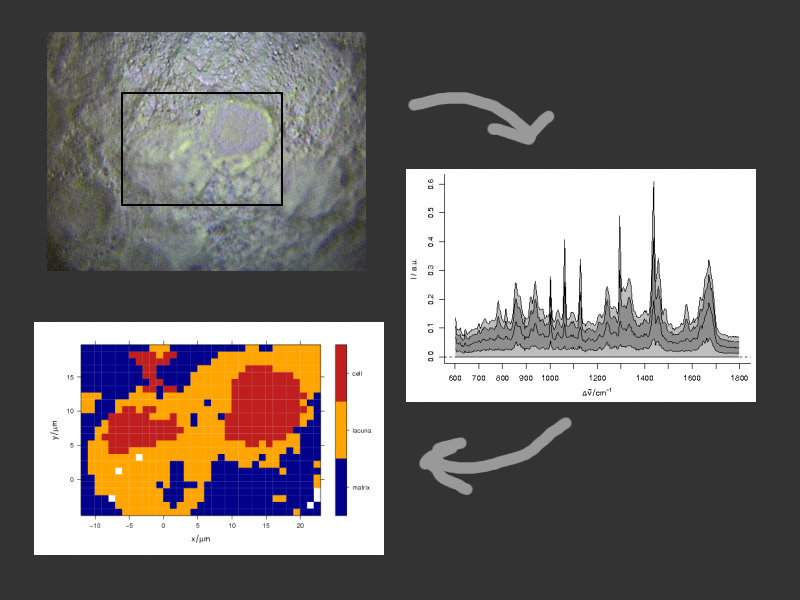
\includegraphics[width=0.5]{hyperSpec_ex}
   {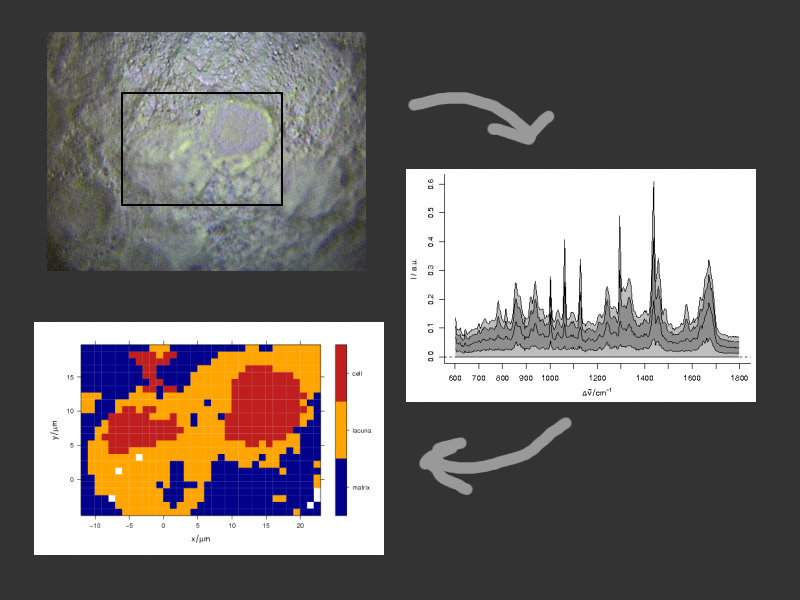
\includegraphics[width=20em]{hyperSpec_ex.png}}
  \end{center}
  
  The spectral data may contain any type of extra data, spatially or time-
resolved information, or conditions.
  \vspace{1em}
 }

%%%%%%%%%%%%%%%%%%%%%%%%%%%%%%%%%%%%%%%%%%%%%%%%%%%%%%%%%%%%%%%%%%%%%%%%%%%%%%
  \headerbox{Large Datasets}{name=model,column=0,below=hyperspec}{
%%%%%%%%%%%%%%%%%%%%%%%%%%%%%%%%%%%%%%%%%%%%%%%%%%%%%%%%%%%%%%%%%%%%%%%%%%%%%%
  \vspace{1em}
  }

%%%%%%%%%%%%%%%%%%%%%%%%%%%%%%%%%%%%%%%%%%%%%%%%%%%%%%%%%%%%%%%%%%%%%%%%%%%%%%
  \headerbox{Fitting}{name=fitting,column=0,below=model}{
%%%%%%%%%%%%%%%%%%%%%%%%%%%%%%%%%%%%%%%%%%%%%%%%%%%%%%%%%%%%%%%%%%%%%%%%%%%%%%
  \vspace{1em}
  }

%%%%%%%%%%%%%%%%%%%%%%%%%%%%%%%%%%%%%%%%%%%%%%%%%%%%%%%%%%%%%%%%%%%%%%%%%%%%%%
  \headerbox{Distance Measure}{name=measure,column=0,below=fitting}{
%%%%%%%%%%%%%%%%%%%%%%%%%%%%%%%%%%%%%%%%%%%%%%%%%%%%%%%%%%%%%%%%%%%%%%%%%%%%%%
  \vspace{1em}
  }

%%%%%%%%%%%%%%%%%%%%%%%%%%%%%%%%%%%%%%%%%%%%%%%%%%%%%%%%%%%%%%%%%%%%%%%%%%%%%%
  \headerbox{Interactive Graphics}{name=results neutralization,column=1,row=0}{
%%%%%%%%%%%%%%%%%%%%%%%%%%%%%%%%%%%%%%%%%%%%%%%%%%%%%%%%%%%%%%%%%%%%%%%%%%%%%%

  With large complex data sets it is not easy, or even possible, to produce a single plot to fully convey the relevant structures and patterns we might want to analyse.  For multi-dimensional data we may wish to have several views of the same data and we would want to visually link these views.  
  \vspace{1em}
  
  Interactive graphics can provide tools for selection which highlight the affected points accross all linked views.  Interactive graphics can also provide a means of enhancing a view dynamically, such as adjusting the visible data range (zooming) about a certain point, to aid in determining precise features.
  \vspace{1em}
  }
%%%%%%%%%%%%%%%%%%%%%%%%%%%%%%%%%%%%%%%%%%%%%%%%%%%%%%%%%%%%%%%%%%%%%%%%%%%%%%
  \headerbox{Footnote}{name=funding,column=1,span=2,above=bottom}{
%%%%%%%%%%%%%%%%%%%%%%%%%%%%%%%%%%%%%%%%%%%%%%%%%%%%%%%%%%%%%%%%%%%%%%%%%%%%%%
  \smaller 
  \hspace{1em}This work was supported in part by Microsoft Research through the European PhD Scholarship Programme.
  }
%%%%%%%%%%%%%%%%%%%%%%%%%%%%%%%%%%%%%%%%%%%%%%%%%%%%%%%%%%%%%%%%%%%%%%%%%%%%%%
  \headerbox{Results (hyperSpecGUI framework)}{name=results,column=1,span=2,below=results neutralization,above=funding}{

  \vspace{1em}
  }
%%%%%%%%%%%%%%%%%%%%%%%%%%%%%%%%%%%%%%%%%%%%%%%%%%%%%%%%%%%%%%%%%%%%%%%%%%%%%%
  \headerbox{Dynamic Workflow}{name=robustness,column=2,row=0,above=results,span=1}{
%%%%%%%%%%%%%%%%%%%%%%%%%%%%%%%%%%%%%%%%%%%%%%%%%%%%%%%%%%%%%%%%%%%%%%%%%%%%%%
  Spectral analysis does not have a single statistical method which can be fitted to the data, workflows are fluid and require investigation of many different techniques.  Usually the workflows would be controlled/dictated/made from the command-line, where at any time you can choose to investigate any particular data or technique.
  \vspace{1em}
  
  {\em hyperSpecGUI} thus provides a collection of widgets which can be invoked at any time and given any data, providing a more intuitive way of interacting with the data while keeping the dynamic characteristics of analysing spectral data.
  \vspace{1em}
  }

%%%%%%%%%%%%%%%%%%%%%%%%%%%%%%%%%%%%%%%%%%%%%%%%%%%%%%%%%%%%%%%%%%%%%%%%%%%%%%
  \headerbox{References}{name=references,column=0,above=bottom}{
%%%%%%%%%%%%%%%%%%%%%%%%%%%%%%%%%%%%%%%%%%%%%%%%%%%%%%%%%%%%%%%%%%%%%%%%%%%%%%
%http://hyperspec.r-forge.r-project.org/
    \smaller
    \vspace{-0.4em}
    \bibliographystyle{ieee}
    \renewcommand{\section}[2]{\vskip 0.05em}
      \begin{thebibliography}{1}\itemsep=-0.01em
      \setlength{\baselineskip}{0.4em}
      \bibitem{amberg07:nonrigid}
        B.~Amberg, S.~Romdhani, T. Vetter.
        \newblock {O}ptimal {S}tep {N}onrigid {ICP} {A}lgorithms for {S}urface {R}egistration
        \newblock In {\em Computer Vision and Pattern Recognition 2007}
      \bibitem{amberg08:recognition}
        B.~Amberg, R.~Knothe, T. Vetter.
        \newblock Expression Invariant Face Recognition with a 3D Morphable Model
        \newblock In {\em Automated Face and Gesture Recognition 2008}
      \end{thebibliography}
  }
%%%%%%%%%%%%%%%%%%%%%%%%%%%%%%%%%%%%%%%%%%%%%%%%%%%%%%%%%%%%%%%%%%%%%%%%%%%%%%
  \headerbox{Open Questions}{name=questions,column=0,span=1,below=measure,above=references}{
%%%%%%%%%%%%%%%%%%%%%%%%%%%%%%%%%%%%%%%%%%%%%%%%%%%%%%%%%%%%%%%%%%%%%%%%%%%%%%
  }

\end{poster}

\end{document}
